\documentclass{article}
\usepackage{graphicx} % Required for inserting images
\usepackage{float}

\title{EV Integration to Ana's Project}
\author{Simon La Vieille}
\date{August 2025}

\begin{document}

\maketitle

\newpage

\section{Introduction}

The Economics of Going Electric in California from Gas to Grid is a project that looks into economics of electrifying residential appliances, with and without the addition of a stand alone PV and battery system. The task of this report was to add another component, cars, and see what their impact of the economics of the household would be. \\

California has the largest population of electric vehicles in the United States, with 35\% of vehicles nationwide in 2023, with 1,256,646 electric vehicle registrations \cite{AlternateFuelsDataCenter}. After more than a century of petroleum dominance, electric vehicles are increasing the popularity as battery cist have declined by almost 90\% over the last decade \cite{TEMPO_NREL}.\\

To be able to add this section to Ana paper, we needed both economic and usage data on electric vehicles (EVs) as well as ICE (internal combustion engine) vehicles to be able to make the comparison.

\section{Load Profiles for EVs}

We first started with EVs, and the required electricity they needed for every day use. To do so, we needed to find the average charging load profiles of electric vehicles in California. Although this was not easy to find, 4 different data sets were investigated, each with their assumptions, upside, and downsides. 

\subsection{TEMPO - NREL}

The first dataset that was investigated was TEMPO: Transportation Energy \& Mobility Pathway Options Model. TEMPO is a comprehensive transportation demand model from the National Renewable Energy Laboratory (NREL) used to explore the long term scenarios fo energy use across the entire United States transportation sector, which generated annual hourly load projection for household EV charging got all counties in contiguous United States until 2050 for a set of vehicle electrification scenarios \cite{TEMPO_Report}. \\

Although this dataset gave access to county specific load profiles, TEMPO assumes that whenever the vehicle is not in use, it is charging. This has two major limitations, first, no time-of-use (TOU) rates decision making can be done, when it is known that many people choose to charge their vehicle when electricity prices are lower, and second, it does not differentiate charging at home versus charging outside. This is a very limiting factor as this study looks at the residence electricity loads

\subsection{EVI Pro - CEC/NREL}

The second possibility was to investigate the dataset used by the CEC and also by NREL. This dataset was used by the AB 2127 \cite{AB2127Report} and the Integrated
Energy Policy Report (IEPR) \cite{IEPRReport} reports written by the California Energy Commission (CEC). Electric Vehicle Infrastructure (EVI) Projection tool has had many versions, starting from EVI-Pro 1, to EVI-Pro 3, going through EVI-Pro Lite. The original EVI-Pro 1 model, developed in 2016 through a collaboration between the CEC and NREL set the standard for estimating the charging demand across California and the US. Then EVI-Pro 2, which was built of the foundation of its predecessor, incorporated evolving technology and market conditions and was used as part of the first AB 2127 assessment published in 2021. EVI-Pro 3 was then upgraded to provide a more realistic depiction of charging behavior, deliver results at a higher level of geographic detail, and address changes in PEV (Plug-in Electric Vehicle) ownership from now to 2035. The EVI-Pro Lite: Load Profile tool estimates EVI power demands on the electric grid for typical daily charging in a given state or city. It is a simplified version of EVI-Pro \cite{EVIPROLite}. Both these versions separated residential, workplace, and dcfc charging. \\

Two issues occurred after thoroughly investigating these options, the first was that both EVI-Pro 2 and 3 were not available to the public, making it inaccessible. The second concerned EVI-Pro Lite which only displayed load profiles for major cities (the difference between these load profiles only depended on the daily driven miles), and did consider the TOU rates. 

\subsection{ISO Data}

The third possibility came from the ISO data \cite{ISO_dataset}. This publicly available dataset encompassed the 8760 of all three utilities in California, namely PG\&E, SCE, and SDG\&E. This data was used with EVI Pro and charge point data in the IEPR report done by the CEC. This dataset gave better granularity than having a general statewide load profile, but could not differentiate between the counties within the same utility. As this data was not simulated, unlike the TEMPO data, TOU rates were considered, making it very interesting to investigate.\\

The major downside of this dataset was that residential demand was not separated from public and workplace charging. As this paper looks into the residential load profile, it made the data very difficult to use.

\subsection{CEC Data}

Finally, the fourth, and chosen dataset was the data used by the CEC in their 2127 report. This data was edited by the CEC for their report using the EVI-Pro 3 data to build a typical day load profile. This dataset therefore considered the fact that people charged with certain TOU rates and is split between residential and non-residential charging.\\

On the other hand, this data is statewide and has only one typical day, meaning no matter what day or where you are located in the state, the analysis will assume you are charging the same way, and the same amount. It also does not differentiate between EV sizes like the TEMPO data does, but is only for light duty EVs, which leads to having an average between plug-in hybrid vehicles (PHEVs) and battery electric (EVs). However, only 12\% of the total are expected to be plug-in hybrids, meaning the curve mostly represents BEVs. This data is unfortunately not publicly available and was sent to a UC-Berkeley colleague for her thesis.\\

\begin{table}[H]
    \centering
    \begin{tabular}{|c|c|c|c|c|c|}\hline
         &  TEMPO&  EVI-Pro 3&  EVI-Pro Lite&  ISO& CEC\\\hline
         Granularity&  County&  County&  Major Cities&  Utility& California\\\hline
         Values&  Per EV&  Per EV&  Per EV&  Per Utility& Per State\\\hline
         Year&  Choice&  Choice&  2030&  Choice& 2030\\\hline
         Access&  full&  none&  full&  full& full\\\hline
         TOU Rates&  No&  Yes&  No&  Yes& Yes\\\hline
         Res/non-res&  Merged&  Split&  Split&  Merged& Split\\\hline
         Car Model&  Option&  Light EVs&  Sedan/SUVs&  Light EVs& Light EVs\\\hline
         8760&  Yes&  2 * 24h&  2 * 24h&  Yes& 24h\\ \hline
    \end{tabular}
    \caption{Dataset Upsides and Downsides}
    \label{DatasetSelection}
\end{table}

Table \ref{DatasetSelection} summarizes the upsides and downsides of each dataset. After having chosen the CEC data load profiles, a daily load profile per vehicle had to be built. The current dataset offered a typical 24 hour load profile per minute for all EVs in California. Therefore, the first step was to divide each value by the fleet size, or 7,100,000 cars, which is the amount of EVs the AB2127 expected to see in 2030. 

\begin{figure}[H]
    \centering
    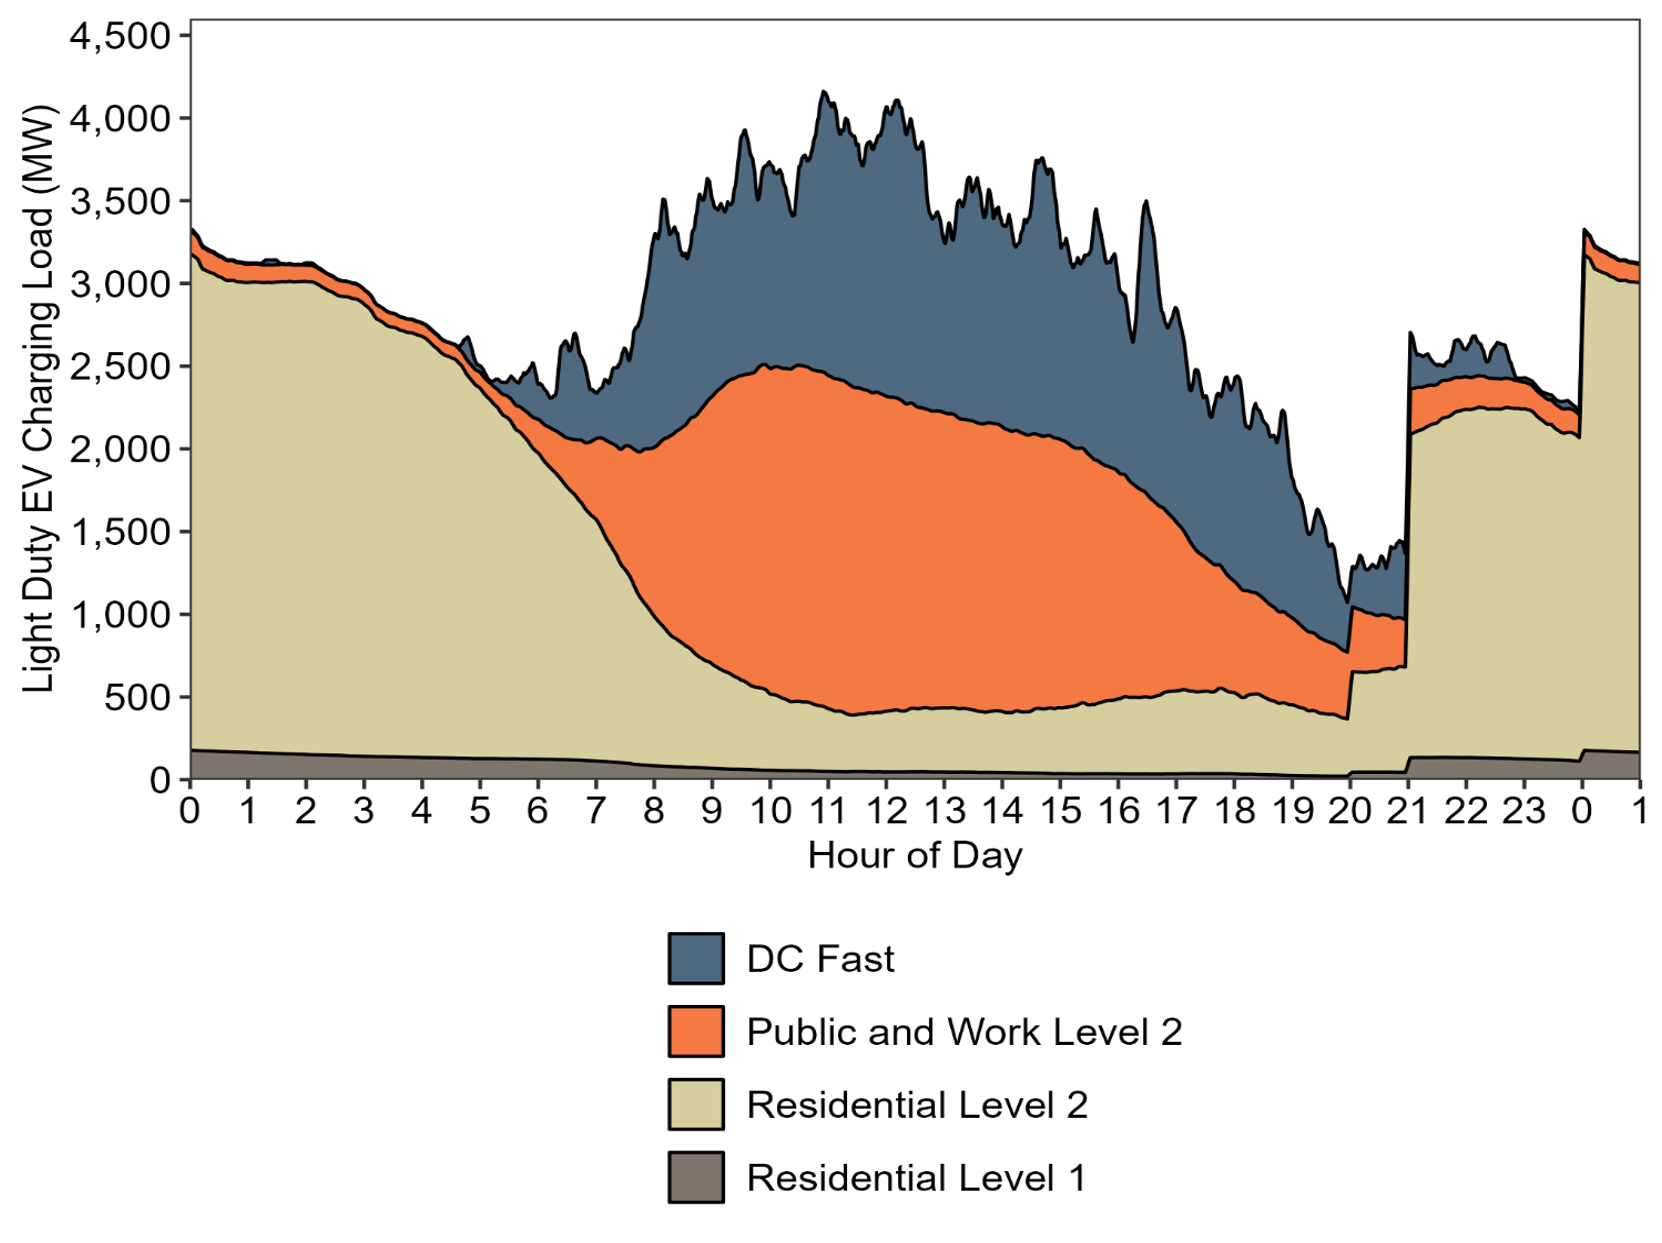
\includegraphics[width=0.9\linewidth]{Figures/DayLoadProfileCEC.png}
    \caption{Daily EV Charging Load (MW) for all vehicles in California in 2030}
    \label{DayLoadProfileCEC}
\end{figure}

\section{Vehicle Costs}

This section aims to explain how the comparison between the costs of owning an ICE or an EV may affect the electrification costs. Both cars have two categories to consider: upfront costs (capital costs and incentives), and recurrent costs (maintenance, fuel, insurance costs).

\subsection{Upfront Costs}
\subsubsection{Capital Costs}
The obvious start is to understand how much an electric vehicle costs compared to its equivalent ICE counter part today. This value depends on many characteristics. To reduce the scope we will only be discussing the costs of battery electric vehicles (not plug-in hybrids). The U.S. department of Energy published a report stating the average costs of different vehicle sizes in 2022 in the United States \cite{CapitalCarCost}. Figure \ref{VehicleCapitalCost2022} shows the price for different size categories of both ICE vehicles and EVs. 

\begin{figure}[H]
    \centering
    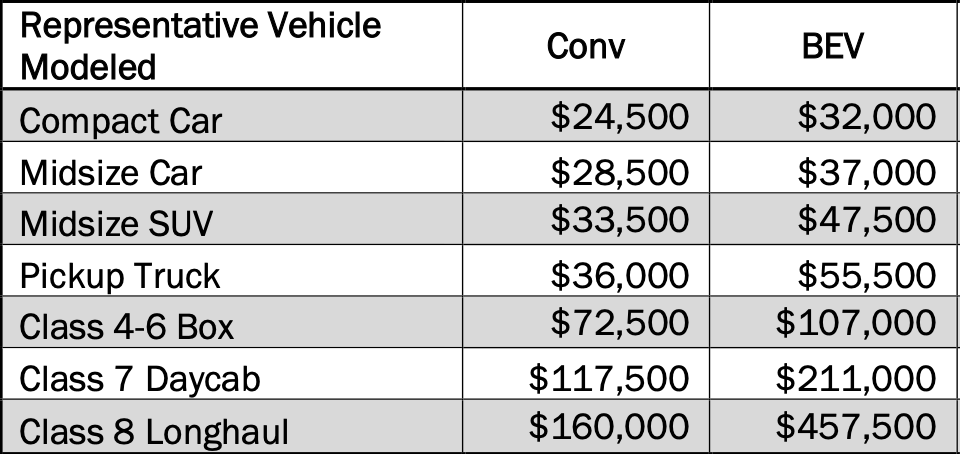
\includegraphics[width=0.75\linewidth]{Figures/VehicleCapitalCost.png}
    \caption{Capital Vehicle Cost for both conventional and battery electric vehicles in 2022 in the US  \cite{CapitalCarCost}}
    \label{VehicleCapitalCost2022}
\end{figure}

However, all of the cost values that will be taken will be for 2023, and not 2022. Therefore as stated bu the US Bureau of Labor Statistics, the Consumer Price Index for all Urban Consumers (CPI-U) increased by 3.4\% \cite{Inflation}. Therefore, table \ref{VehicleCapitalCost2023} shows the real capital cost values, after having applied the inflation rate.\\

\begin{table}[H]
    \centering
    \begin{tabular}{|c|c|c|}\hline
         Vehicle Modeled&  Conv& BEV\\\hline
         Compact Car&  \$25,333& \$33,088\\\hline
         Midsize Car&  \$29,469& \$38,258\\\hline
         Midsize SUV&  \$34,639& \$49,115\\\hline
         Pickup Truck&  \$37,224& \$57,387\\\hline
         Class 4-6 Box&  \$74,965& \$110,638\\\hline
         Class 7 Daycab&  \$121,495& \$218,174\\\hline
         Class 8 Longhaul&  \$165,440& \$473,055\\ \hline
    \end{tabular}
    \caption{Updated Capital Vehicle Cost for both conventional and battery electric vehicles in 2023 in the US}
    \label{VehicleCapitalCost2023}
\end{table}

As the date that has been chosen will merge level 1 and level 2 residential charging, it is also important to consider the installation cost of level 2 charging at home, which allows for faster vehicle charging. The charging curve shows that most of the residential charging comes from level 2. Therefore, it was found from the United States department of transportation, that the installation cost of an L2 charger as well as the outlet would be around \$1400 \cite{L2ChargerCost}.

\subsubsection{Incentives}

With this comes the incentives that are present when purchasing a new electric vehicle. There are two types of incentives for both chargers and EVs, one is income eligible, and the other is not. The table \ref{EV Incentives} summarizes the start/end date, and value of these incentives, assuming the vehicle is purchased new \cite{DriveClean}.

\begin{table}[H]
    \centering
    \begin{tabular}{|c|c|c|c|c|}\hline
         &  \multicolumn{2}{|c|}{Charger}&  \multicolumn{2}{|c|}{Vehicle} \\\hline
         &  Federal&  State&  Federal& State\\\hline
         Value&  30\%; max \$1,000&  \$2,000&  \$7,500& \$12,000\\\hline
 Income Based& No& Yes& No&Yes\\\hline
         End-date&  12/31/32&  N.a.&  09/30/25& N.a.\\ \hline
    \end{tabular}
    \caption{Incentives for purchasing an electric vehicle and corresponding chargers.}
    \label{EV Incentives}
\end{table}

\subsection{Recurrent Costs}

Finding the value of the recurrent costs has shown the necessity of finding the Vehicles Miles Traveled (VMT). The Federal Highway Administration gives us the number of vehicles in California to be 31,119,113 as of 2022 \cite{NumberVehiclesCalifornia}, and also gives us in a separate table the total VMT driven by all these vehicles in a single year, 315,244 million miles per year \cite{TotalVMTCalifornia}. By diving the two, we get a per vehicle VMT of 10,130 miles driven per year.

\subsubsection{Maintenance Costs}

The first recurrent costs when purchasing a car are the maintenance costs. These occur to keep the vehicle running in good condition. As the components of electric vehicle and ICE vehicles are different, their maintenance costs will also vary (car battery in EVs for instance). \\

According to the international council on clean transportation \cite{Maintenance/InsuranceCosts}, in 2021, the maintenance costs of a new electric vehicle was of 0.012 \$/mile, and of 0.028 \$/mile for a new conventional vehicle. By multiplying this value by the VMT per vehicle per year, we get that electric vehicles spend \$121.6/year of maintenance costs compared to \$283.6/year for ICE vehicles, assuming the same distance is driven no matter the vehicle in California.

\subsubsection{Insurance Costs}

Similarly, the international council on clean transportation also gives us the insurance price per vehicle per month \cite{Maintenance/InsuranceCosts} to be 170\$/month for EVs and \$153/month of ICE vehicles, leading to \$2040/year for EVs and \$1836/year for conventional vehicles. 

\subsubsection{Fuel Costs}

As was presented earlier, the daily load profile will give us that amount. However, as also mentioned, only levels 1 and 2 residential charging was considered for the residential load profile, but a large share of the charging also occurs at the workplace/public, and on DC fast chargers. Using python, and knowing the average rate of DC fast chargers as well as public level 2 of \$0.40/kWh and \$0.30/kWh respectively \cite{DriveClean}, we found the average yearly constant amount of money spent charging outside of home. The fleet size is of 7,100,000 EVs. 

\begin{table}[H]
    \centering
    \begin{tabular}{|c|c|c|}\hline
         &  Public/Work Charging L2& DC Fast Charger\\\hline
         kWh/vehicle/day&  2.76& 2.33\\\hline
         Dollar/kWh&  0.30& 0.40\\\hline
 \$/vehicle/year& 301.85&340.69\\\hline
    \end{tabular}
    \caption{Costs of Charging in Public}
    \label{DCFC/publiccharging}
\end{table}

As for the fuel costs of ICE vehicles, the average state values updated daily by AAA were used and imported in the python code to make the recurrent cost of fuel be county dependent \cite{AAAFuelPrices}.

\section{Utility Updated Costs and Efficiencies}

\subsection{Solar}

Regarding solar costs, Ana had found values of around \$2800/kW. The CPUC on the other hand produced a report stating that there is a large discrepancy between values. The NREL Annual Technology Baseline value of \$2.34/W seemed very low while the Tracking the Sun report estimated a value of \$3.80/W in 2019 which seemed very high. Therefore, the commission found that a value of \$3.30 per watt to be reasonable as the adopted 2023 cost of solar in California, and account for electrical panel upgrades, delays, and the current inflationary costs \cite{CostofSolar}.

\subsection{Battery}

On the other hand, the CEC published a report \cite{CECStorage} in which they used the default storage costs based on NREL's ATB 2022 data, meaning the national average, showing that the national average was good enough to be used for state specific reports. Therefore, this report will use NREL ATB data \cite{ATB2024}, following the moderate scenario which assumes "Innovations observed in today's market become more widespread, and innovations nearly market-ready today come into the market. Current levels of public and private R\&D investment continue. This scenario may be considered the expected level of technology innovation". This scenario says that the installation cost of residential batteries of 5kW/12.5kWh will be of \$18,258 in 2023. 

\subsection{Heat Pump Water Heater}

The following counties are missing, and it has been decided to take the state median to fill in the gaps. There are 13 Californian counties missing from the list. Here are the parameters chosen from the TECH data in terms of water heater:

\begin{itemize}
    \item Building Type: Single Family
    \item Installed Equipment Description: 
    \begin{itemize}
        \item Heat Pump Water Heater
        \item Split System HPWH
        \item 120V integrated HPWH
        \item 240V integrated HPWH
    \end{itemize}
\end{itemize}

The output that have been investigated are the following, which have been displayed per county. The county median is displayed in a csv file.

\begin{itemize}
    \item Total Project Cost per Unit (\$)
    \item Total Incentive Received by Contractor (\$)
    \item Uniform Energy Factor
\end{itemize}

In the case where some counties are missing data, it was decided to use the state median to fill in those gaps. It is important to note that these are the contractor costs, meaning the turnkey costs.

\subsection{Heat Pump - Space Heater}

Similarly for space heaters, we have certain counties missing, 5 in total. Once again, In the case where some counties are missing data, it was decided to use the state median to fill in those gaps. 

As a lot of data was missing, specifically the Uniform Energy Factor which is rarely displayed in the TECH data for space heaters, it was decided to take into account all of the heat pumps that did required duct, meaning all AHRI types with no -O suffix. Once again, the output that have been investigated are the following, which have been displayed per county. The county median is displayed in a csv file. It is important to note that these are the contractor costs, meaning the turnkey costs.

\begin{itemize}
    \item Total Project Cost per Unit (\$)
    \item Total Incentive Received by Contractor (\$)
    \item Uniform Energy Factor
\end{itemize}

\subsection{Rest of the Values}

The gas, electric cooking values, as well as the gas water and air heater could not be taken from the TECH data, so following Cristina's approach, this paper uses the appliance comparison value from the California Air Resources Board \cite{ApplianceCost}. The following table shows the cost split, with the 3.4\% inflation rate, as the values are from 2022, and the paper discusses the 2023 costs\cite{Inflation}. It is important to note that these are the contractor costs, meaning the turnkey costs.

\begin{table}[H]
    \centering
    \begin{tabular}{|c|c|c|c|c|c|}\hline
         COSTS&  Capital&  Installation&  Other&Total 2022 &Total 2023\\\hline
         Induction Stove&  \$2400&  \$1380&  \$340& \$4120&\$4260.08\\\hline
         Gas Stove&  \$1600&  \$890&  \$220& \$2710&\$2802.14\\\hline
         Gas Water Heater&  \$900&  \$1200&  \$90& \$2190&\$2264.46\\\hline
 Gas HVAC& \$4500& \$4180& \$770& \$9450&\$9771.3\\ \hline
    \end{tabular}
    \caption{Costs of Appliances}
    \label{ApplianceCosts}
\end{table}

Finally, regarding the induction stove, it was found they are 85\% efficient \cite{InductionEfficiency}, making them up to three more times efficient than their gas counterpart \cite{InductionEfficiencyvs}. 

\subsection{Lifetimes}

The EIA produced a report in 2023 looking at the average lifetime for all components \cite{EIALifetimes}. The following tables resumes the lifetime found in the report. Ana has chosen to take an average of 15 years, as all values are around that timeline, making the payback period easier to compute

\begin{table} [H]
    \centering
    \begin{tabular}{|c|c|}\hline
         &  Lifetime\\\hline
         Induction Stove&  17\\\hline
         Gas Stove&  15\\\hline
         Electric Water Heater&  15.1\\\hline
         Gas Water Heater&  14.5\\\hline
         Electric Heat Pump&  15.3\\\hline
         Gas Heat Pump&  12-18\\ \hline
    \end{tabular}
    \caption{Lifetime of Residential Components}
    \label{LifetimesComponents}
\end{table}

\newpage

\bibliographystyle{unsrt}
\bibliography{reference}        

\end{document}
